\documentclass{beamer}
\usepackage[utf8]{inputenc}

\usetheme{Madrid}
\usecolortheme{default}
\usepackage{amsmath,amssymb,amsfonts,amsthm}
\usepackage{txfonts}
\usepackage{tkz-euclide}
\usepackage{listings}
\usepackage{adjustbox}
\usepackage{array}
\usepackage{tabularx}
\usepackage{gvv}
\usepackage{lmodern}
\usepackage{circuitikz}
\usepackage{tikz}
\usepackage{graphicx}
\usepackage{amsmath}
\usepackage{mathtools}
\setbeamertemplate{page number in head/foot}[totalframenumber]

\usepackage{tcolorbox}
\tcbuselibrary{minted,breakable,xparse,skins}



\definecolor{bg}{gray}{0.95}
\DeclareTCBListing{mintedbox}{O{}m!O{}}{%
  breakable=true,
  listing engine=minted,
  listing only,
  minted language=#2,
  minted style=default,
  minted options={%
    linenos,
    gobble=0,
    breaklines=true,
    breakafter=,,
    fontsize=\small,
    numbersep=8pt,
    #1},
  boxsep=0pt,
  left skip=0pt,
  right skip=0pt,
  left=25pt,
  right=0pt,
  top=3pt,
  bottom=3pt,
  arc=5pt,
  leftrule=0pt,
  rightrule=0pt,
  bottomrule=2pt,
  toprule=2pt,
  colback=bg,
  colframe=orange!70,
  enhanced,
  overlay={%
    \begin{tcbclipinterior}
    \fill[orange!20!white] (frame.south west) rectangle ([xshift=20pt]frame.north west);
    \end{tcbclipinterior}},
  #3,
}
\lstset{
    language=C,
    basicstyle=\ttfamily\small,
    keywordstyle=\color{blue},
    stringstyle=\color{orange},
    commentstyle=\color{green!60!black},
    numbers=left,
    numberstyle=\tiny\color{gray},
    breaklines=true,
    showstringspaces=false,
}


\title 
{5.3.17}



\author 
{Pratik R-AI25BTECH11023}



\begin{document}


\frame{\titlepage}
%------------------------------------
\begin{frame}{Question}
Solve the system of linear equations using the matrix method 
\begin{align}
    7x+2y=11 \\
    4x-7y=2
\end{align}
\end{frame}
\begin{frame}{Solution}
Using augmented matrix
\begin{align}
   \myvec{7 & 2 &\vrule &11 \\
   4 & -7 &\vrule &2}
\end{align}
Reducing it to reduced echelon form
\begin{align}
    \myvec{7 & 2 &\vrule &11 \\
   4 & -7 &\vrule &2} \xleftrightarrow{R_2 = R_2- \frac{4}{7} R_1 } \myvec{7 & 2 &\vrule &11 \\
   0 & -\frac{57}{7} &\vrule &-\frac{30}{7}}
\end{align}
\end{frame}
\begin{frame}{Solution}
\begin{align}
\xleftrightarrow{R_2= \frac{14}{57} R_2 } \myvec{7 & 2 &\vrule &11 \\
   0 & -2 &\vrule &-\frac{60}{57}}
    \xleftrightarrow{R_1 = R_1+ R_2} \myvec{7 & 0 &\vrule &\frac{567}{57} \\
   0 & -2 &\vrule &-\frac{60}{57}} 
\end{align}
\begin{align}
    \xleftrightarrow{R_1 = R_1/7} \myvec{1 & 0 &\vrule &\frac{81}{57} \\
   0 & -2 &\vrule &-\frac{60}{57}} \xleftrightarrow{R_2 = R_2/-2} \myvec{1 & 0 &\vrule &\frac{81}{57} \\
   0 & 1 &\vrule &\frac{30}{57}} 
\end{align}
\end{frame}
\begin{frame}{Solution}
Hence 
\begin{align}
    \myvec{x \\y} = \frac{1}{57} \myvec{81\\30}
\end{align}
\end{frame}
\begin{frame}{plot}
\centering
    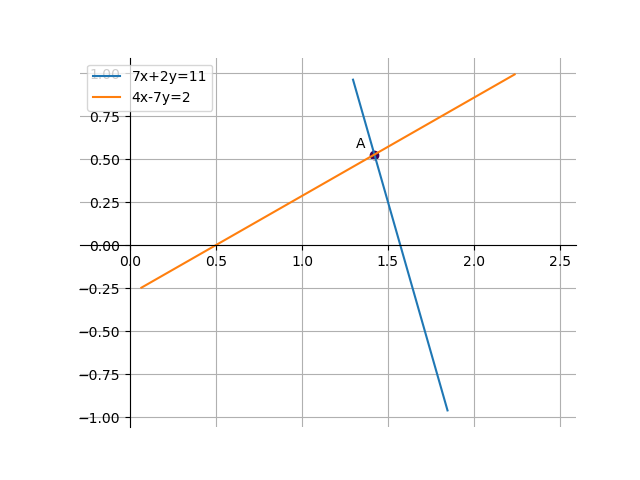
\includegraphics[width=\columnwidth, height=0.8\textheight, keepaspectratio]{../figs/fig.png}     
\end{frame}


\end{document}
